\documentclass[tikz,border=5pt]{standalone}
\usepackage{tikz}
\usetikzlibrary{positioning,fit,backgrounds,calc,arrows.meta}
\usepackage{xcolor}

\definecolor{gitopsblue}{RGB}{51,108,229}
\definecolor{manualgray}{RGB}{102,102,102}
\definecolor{okgreen}{RGB}{76,175,80}
\definecolor{driftred}{RGB}{229,115,115}

\begin{document}
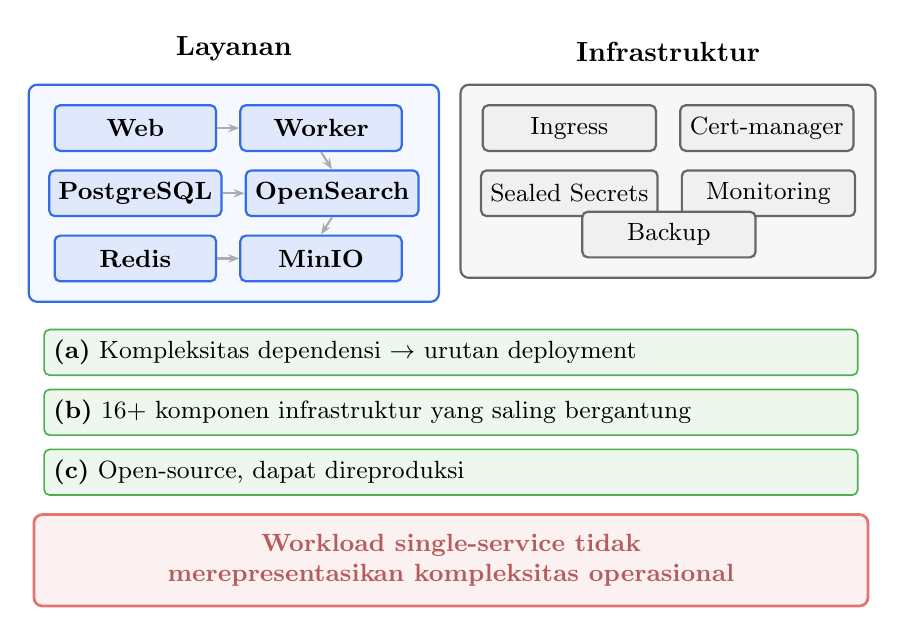
\begin{tikzpicture}[
    svc/.style={rectangle, rounded corners=2pt, draw=gitopsblue, fill=gitopsblue!15,
                minimum width=2.05cm, minimum height=0.58cm, align=center,
                line width=0.8pt, font=\small\bfseries},
    infra/.style={rectangle, rounded corners=2pt, draw=manualgray, fill=manualgray!10,
                  minimum width=2.2cm, minimum height=0.58cm, align=center,
                  line width=0.8pt, font=\small},
    criteria/.style={rectangle, rounded corners=2pt, draw=okgreen, fill=okgreen!10,
                     text width=10.1cm, minimum height=0.58cm, align=left,
                     line width=0.6pt, font=\small},
    arrow/.style={-{Stealth[length=4pt]}, line width=0.75pt, draw=gray!65}
]

\node[svc] (web) {Web};
\node[svc, right=0.28cm of web] (worker) {Worker};
\node[svc, below=0.22cm of web] (pg) {PostgreSQL};
\node[svc, right=0.28cm of pg] (os) {OpenSearch};
\node[svc, below=0.22cm of pg] (redis) {Redis};
\node[svc, right=0.28cm of redis] (minio) {MinIO};

\draw[arrow] (web) -- (worker);
\draw[arrow] (pg) -- (os);
\draw[arrow] (redis) -- (minio);
\draw[arrow] (worker.south) -- (os.north);
\draw[arrow] (os.south) -- (minio.north);

\node[infra, right=1.0cm of worker] (ingress) {Ingress};
\node[infra, right=0.28cm of ingress] (cert) {Cert-manager};
\node[infra, below=0.22cm of ingress] (sealed) {Sealed Secrets};
\node[infra, right=0.28cm of sealed] (monitor) {Monitoring};
\node[infra, below=0.22cm of $(sealed)!0.5!(monitor)$] (backup) {Backup};

\begin{scope}[on background layer]
    \node[rectangle, rounded corners=3pt, draw=gitopsblue, fill=gitopsblue!5,
          inner sep=7pt, line width=0.8pt, fit=(web)(worker)(pg)(os)(redis)(minio)] (svcgrp) {};
    \node[rectangle, rounded corners=3pt, draw=manualgray, fill=manualgray!5,
          inner sep=7pt, line width=0.8pt, fit=(ingress)(cert)(sealed)(monitor)(backup)] (infragrp) {};
\end{scope}

\node[font=\normalsize\bfseries, above=0.16cm of svcgrp.north] {Layanan};
\node[font=\normalsize\bfseries, above=0.16cm of infragrp.north] {Infrastruktur};

\coordinate (topcenter) at ($(svcgrp.south)!0.5!(infragrp.south)$);
\node[criteria, below=0.48cm of topcenter] (c1) {
    \textbf{(a)} Kompleksitas dependensi $\rightarrow$ urutan deployment
};
\node[criteria, below=0.16cm of c1] (c2) {
    \textbf{(b)} 16+ komponen infrastruktur yang saling bergantung
};
\node[criteria, below=0.16cm of c2] (c3) {
    \textbf{(c)} Open-source, dapat direproduksi
};

\node[rectangle, rounded corners=3pt, draw=driftred, fill=driftred!10,
      inner sep=7pt, line width=1pt, below=0.22cm of c3,
      text width=10.1cm, align=center, font=\small\bfseries, text=driftred!80!black] (arg) {
    Workload single-service tidak\\
    merepresentasikan kompleksitas operasional
};

\end{tikzpicture}
\end{document}
